% HIER BITTE AUSFÜLLEN:

\newcommand{\abschlussarbeit}{Studienarbeit} % Bachelorarbeit / Masterarbeit
\newcommand{\zweitpruefer}{Prof. Dr. Erika Mustermann} % Zweitprüfer

\newcommand{\sprache}{german} % Deutsch: german / Englisch: english
\newcommand{\druck}{oneside} %  / Simplex: oneside / Duplex: twoside

\newcommand{\titel}{Predictive Analytics \\
                    Daily Financial News for 6000+ Stocks}

\newcommand{\nameFirst}{Benjamin Kasten}
\newcommand{\nameSecond}{Dominik Höhr}
\newcommand{\matrikelnummerFirst}{7154784}
\newcommand{\matrikelnummerSecond}{7157684}
\newcommand{\adresseFirst}{Warburger Str. 100, 33098 Paderborn}
\newcommand{\adresseSecond}{Warburger Str. 100, 33098 Paderborn}
\newcommand{\upbmailFirst}{bkasten@mail.uni-paderborn.de}
\newcommand{\upbmailSecond}{dhoehr@mail.uni-paderborn.de}
\newcommand{\abgabedatum}{15. August 2020}


% % % % % % % % % % % % % % % % % % % % % % % % % % % % % % % % % % % % % % %


\documentclass[fontsize=12pt,BCOR=15mm,DIV=15,a4paper,headsepline,headings=small,\druck,openright,appendixprefix]{scrbook}

\usepackage[onehalfspacing]{setspace}
\raggedbottom
\usepackage{emptypage}
\makeatother 
\usepackage{parskip}

\usepackage{hyperref}
\usepackage[utf8]{inputenc} % Zeichenkodierung
\usepackage[T1]{fontenc} % Trennung von Wörtern mit Umlauten
\usepackage{lmodern} % Latin Modern font benutzen (enhanced computer modern clone, serif)
\usepackage[\sprache]{babel} % Dokument in deutsch inklusive Silbentrennung nach neuer deutscher Rechtschreibung
\usepackage{natbib} % Stil für Literaturverzeichnis
\usepackage{amsmath} % verbesserte mathematische Umgebung
\usepackage{amsfonts} % zusätzliche mathematische Zeichen
\usepackage{amssymb} % zusätzliche mathematische Zeichen
\usepackage{amsthm} % zusätzliche mathematische Zeichen
\usepackage[hyphens]{url}
\usepackage{exscale} % Anpassung mathematischer Symbole an die Schriftgröße
\usepackage{amstext} % \text in mathematischer Umgebung
\usepackage{array} % Tabellen
\usepackage{rotating} % rotierte Tabellen und Bilder
\usepackage[algoruled, algochapter]{algorithm2e} % Pseudocode
\usepackage{verbatim} % Funktion zum Schreiben von unformatiertem Text
\usepackage[section]{placeins} % Verhindert das Wandern von floats in eine andere section
\usepackage{color} % Farbiger Text
\usepackage{graphicx} % Funktionen zum Einfügen von Bildern
\usepackage{subfigure} % Anzeigen von Bildern aus mehreren Einzelbildern
\usepackage{setspace} % Einstellen des Zeilenabstandes
\usepackage[urlcolor = black,plainpages=false,pdfpagelabels=true,colorlinks=true,linkcolor=black,citecolor=black,bookmarksopen=true]{hyperref} % Verweise werden im PDF zu Hyperlinks
\usepackage{scrlayer-scrpage} % Koma für Kopfzeilen-Formatierung
\usepackage[nounderscore]{syntax}
\usepackage{tabulary} % bessere Tabellen
\usepackage{tabularx} % bessere Tabellen
\usepackage{longtable} % für Tabellen über mehrere Seiten
\usepackage{array}
\usepackage{paralist} % für kleine Einzüge mit \setdefaultleftmargin{0.5em}{}{}{}{}{}
\usepackage{booktabs}
\usepackage{multirow}
\usepackage[table,xcdraw]{xcolor}
\usepackage[hang]{footmisc} %Große Zahlen in Fußnoten
\usepackage{url}
\usepackage[center]{caption}
\makeatletter
\def\@makefnmark{\hbox{\textsuperscript\@thefnmark}}
% \ohead{\leftmark} %Only chapter in header (not section!)
\makeatother
\let\footnotesize\small

\bibliographystyle{apalike} % Literaturverzeichnis entsprechend DIN 1505 formatiert, allerdings ohne URL und ISBN
\renewcommand{\topfraction}{0.85} % Anteil einer Seite, die von Floats belegt sein darf (default 0.7)
\renewcommand{\textfraction}{0.1} % Anteil einer Seite, die mindestens Text sein muss (default 0.2)
\renewcommand{\floatpagefraction}{0.75} % Anteil einer Seite, die ein Float einnehmen darf, ohne auf die nächste Seite gesetzt zu werden (default 0.5)

\usepackage{lipsum}

% Begin
\begin{document}

% Front Matter
\pagestyle{empty}
\pagenumbering{alph}

\vfil

\begin{titlepage}

        \begin{center}
        	
\includegraphics[scale=1.]{img/data_analytics_group.png}
        \end{center}
        
        \vspace{8ex}
        
        \begin{center}
            
            Universität Paderborn\\
            Fakultät für Wirtschaftswissenschaften\\
            Department Wirtschaftsinformatik\\
            
            \vspace{8ex}
            
            \Large
            \abschlussarbeit\\
            
            \vspace{7ex}
            
            \textbf{\sffamily{\titel}}
            
            \vspace{7ex}
            
            \normalsize
            
            by\\
            \name\\
            Matrikelnummer:~\matrikelnummer\\
            \adresse\\
            \upbmail\\
            
            \vspace{8ex}
            
            vorgelegt bei\\
            Prof. Dr. Oliver Müller\\
            \zweitpruefer\\
            
            \vspace{10ex}
            
            \abgabedatum
            
        \end{center}
        
    \end{titlepage}
    
\vfil 
\cleardoublepage

\noindent
\section*{Eidesstattliche Erklärung}

Hiermit erkläre ich, \nameFirst, an Eides statt, dass ich die vorliegende Arbeit selbstständig, ohne fremde Hilfe und ohne Benutzung anderer als der angegebenen Hilfsmittel angefertigt habe. Die aus fremden Quellen (einschließlich elektronischer Quellen) direkt oder indirekt übernommenen Gedanken, Tabellen, Skizzen, Zeichnungen, bildliche Darstellungen usw. sind ausnahmslos als solche kenntlich gemacht. Die Arbeit ist in gleicher oder ähnlicher Form oder auszugsweise im Rahmen einer anderen Prüfung noch nicht vorgelegt worden.

\bigskip

Paderborn, den \abgabedatum

\begin{flushright}
\bigskip
\bigskip
\bigskip

------------------------------------------- \\
\nameFirst
\end{flushright}

\section*{Eidesstattliche Erklärung}

Hiermit erkläre ich, \nameSecond, an Eides statt, dass ich die vorliegende Arbeit selbstständig, ohne fremde Hilfe und ohne Benutzung anderer als der angegebenen Hilfsmittel angefertigt habe. Die aus fremden Quellen (einschließlich elektronischer Quellen) direkt oder indirekt übernommenen Gedanken, Tabellen, Skizzen, Zeichnungen, bildliche Darstellungen usw. sind ausnahmslos als solche kenntlich gemacht. Die Arbeit ist in gleicher oder ähnlicher Form oder auszugsweise im Rahmen einer anderen Prüfung noch nicht vorgelegt worden.

\bigskip

Paderborn, den \abgabedatum

\begin{flushright}
\bigskip
\bigskip
\bigskip

------------------------------------------- \\
\nameSecond
\end{flushright}
\cleardoublepage

\section*{Abstrakt}

@bkasten füg mal bitte das Exposé hier ein!

\textbf{Stichworte:} data science, machine learning
\cleardoublepage

\pagestyle{scrheadings}
\clearscrheadfoot
\ohead{\headmark}
\ofoot{\pagemark}

\frontmatter

\tableofcontents
\cleardoublepage

\listoffigures
\cleardoublepage

\listoftables
\cleardoublepage

% Thesis
\mainmatter
\chapter{Business Understanding}

% Hier soll das Problem erklärt werden, was bereits gemacht wurde und was von uns als nächstes getan wird
\section*{Motivation}
Seit der Digitalisierung und dem Zugang zum Internet für den Großteil der Weltbevölkerung werden Nachrichten fast schon in Echtzeit auf Onlineportalen veröffentlicht und frei zugänglich gemacht. So ist es jeder Person mit Internetzugang möglich, aktuelle Nachrichten fast ohne Zeitverzug parallel zu einer riesigen Menge anderen Menschen zu konsumieren. Darunter fallen auch Nachrichten bezüglich Aktien (im Folgenden Aktiennews). Aktiennews sind Nachrichten, die sich mit der Entwicklung von Aktienpreisen beschäftigen. Zu einer Aktiennews gibt es immer eine Headline. In dieser Headline versuchen die Autor:innen des Artikels, das Thema der Nachricht kurz und knapp zu beleuchten und zusammenzufassen. So beinhalten viele Headlines bspw. die Änderung des Aktienpreises und das zugehörige Unternehmen. Durch die Headline wissen die Besucher:innen eine Nachrichtenportals, wie sich ein Aktienkurs entwickelt, ohne den gesamten Artikel lesen zu müssen. Menschen, die in Aktien, ETFs etc. investieren und Aktiennews lesen, reagieren möglicherweise direkt auf die aktuelleste Headline, ohne den Artikel dazu zu lesen. Beispielsweise kann auf eine negative Headline zu einem Unternehmen, dessen Aktien ein Kunde besitzt, zum schnellen Verkauf dieser führen. Positive Nachrichten könnten zu einem Anstieg der Nachfrage nach den Aktien des Unternehmens führen und somit dessen Wert erhöhen.\\
Warum sollte jetzt ein Computer scih damit beschäftigen, Artikelheadlines zu analysieren, und zu bewerten, ob sich der Aktienkurs der in der Headline genannten Unternehmen verändern könnte? Natürlich könnten auch Menschen sich die Headlines durchlesen, und entsprechend darauf reagieren, bspw. mit einem Kauf oder Verkauf der Aktie. Jedoch können Computer um einiges schneller texte lesen, und somit auch schneller reagieren. Ein Computer kann also diese Arbeit für den Menschen übernehmen, und somit seinen Erfolg als Anleger:in erhöhen.
\section*{Forschungsfrage}
Wir wollen untersuchen, ob es einen Zusammenhang zwischen des Sentiment der Headlines gibt und dem Aktienkurs nach der Veröffentlichung der Headline. Falls ja, wann (zeitlich) lässt sich ein Effekt am stärksten feststellen? Lässt sich also anhand des Senitments einer Headline der Aktienkurs einer dieser Headline zu einem bestimten Zeitpunkt vorhersagen?
\section*{Verwandte Literatur}
Das Thema Stock Price Prediction hat in der LIterratur in den letzen Jahren einen großen Zuwachs bekommen. Hier listen wir einige Quellen auf, die in Zusammenhang mit unserem Forschungsthema stehen.\\
Lárló Nemes, Attila Kiss (2021) haben vier verschiedene Ansätze zur Sentiment Analyse von Economic News genutzt. Um die verschiedene Ansätze vergleichen zu können, wurde zu erst BERT genutzt, und dann die Tools Vader, Textblob und ein RNN. Es hat sich herausgestellt, dass BERT und RNN im Vergleich zum Vader Tool und Textblob deutlich einen deutlich besseren Senitment Score ermitteln konnten, ohne neutrale Ergebnisse. Daraufbasierend konnte durch den Abgelich des Senitments und der Stockpriceentwicklung der Moment festgestellt werden, der den Effekt der Haedline auf den Aktienkurs abbildet.\\
Arul Agarwar (2020) hat mit Hilfe des Python Tools VADER eine Analyse der Nachrichten von einzelnen Unternehmen vorgenommen. Es wurden ganze HTML Seiten heruntergeladen,aus diesen die bwichtigen Informationen herausgefiltert. Dann wurde ein wörterbuchbasierter Ansatz mithilfe des VADER Tools verwendet, um den einzelnen Nachrichten eine Sentiment Score zuzuweisen. Dem VADER LExicon wurden zudem weitere Wörter hinzugefügt bzw. das Sentiment geändert, um eine Missinterpretation (wegen dem Finanzmarkt) zu verhinden. Zwischen dem Sentiment der Nachrichten dem Stock Price konnte eine starke Korrelation erkannnt werden, die spätestens am nächsten Werktag auftrat.
\section*{Nächste Schritte}
\chapter{Data Understanding}

Überschriften mit Zeitstempeln
\chapter{Data Preparation}
Verbleibend sind die unbereinigten Überschriften.
Außerdem ist bereits auffällig geworden, dass eine möglich Zielvariable im vorhanden Datensatz fehlt. Alle vorliegenden Daten sind bislang unbewertet. Im Sinne unserer Forschungsfrage gilt es im Schritt der Konstruktion der Daten die entsprechende Zielvariable zu evaluieren und zu ergänzen, um so eine geeignete Bewertung bzw. Gewichtung der Überschriften herleiten zu können.
Als Zielvariable erscheint der Aktienkurs geeignet. Dieser bietet ein objektives Abbild des Wertes der Aktie zum gegebenen Zeitpunkt. Somit verbleibt es dem Modell eine Verbindung zwischen der Veröffentlichten Headline und der Veränderung des Aktienkurses herzustellen.

\section*{Bereinigen}
Aufgrund der Beschränkungen durch die kostenfreie Version, der zugrunde Liegenden API, zur Ergänzung der Aktienpreise zu den entsprechenden Headlines, sind wir gezwungen den Datensatz auf die letzten Zwei Jahre zu verkürzen.
Dies hat kein semantischen Auswirkungen. Nicht abzustreiten, das entsprechende Modell würde ungemein genauer werden, wenn mehr historische Daten zur Verfügung stehen würden. Doch semantisch stellt die Anzahl der verwendeten Einträge und Insbesondere die Anzahl der verwendeten Stocks keinen Einflussfaktor dar, es werden keine möglichen Predictoren entfernt. Auf der anderen Seite allerdings ist es durchaus möglich dass das Modell, aufgrund des starken und schnellen Wandels des Aktienmarktes, eine zeitlich begrenzte Gültigkeit besitzt. \\
Denkbar ist eine Gewichtung des Einflusses von Headlines auf Aktien, welche nur sehr wenig oder sehr oft, über einen längeren Zeitraum, erwähnt werden. Dies ist sicherlich ein Interessantes Forschungsthema, jedoch nicht Teil dieser Arbeit.\\
Da nur 4\% der Daten Uhrzeiten beinhalten, werden die Zeitstempel auf Tage reduziert. Somit ist nur eine tagesgenaue vorhersage möglich.
Nach der Bereinigung der Daten besteht der Datensatz nun mehr aus rund 164698 Einträgen mit einer Zeitspanne vom 21.August 2019 bis zum 11.Juni 2021.\\

\section*{Konstruieren}
Wie einleitend schon erwähnt gilt es nun die Zielvariable zu ergänzen. Hierfür nutzen wir eine API die zu den jeweiligen Aktienkennungen (Ticker) die entsprechenden Aktienpreise liefert. Bei Angabe des Tickers, eines Zeitraumes und eines Intervalls, erhält man jeweils die Börsenpreise zu Börsenbeginn (open), Börsenschluss (close), den Maximalpreis (high) und den Tiefspreis (low) zum entsprechenden Zeitpunkt. \\Verwendet wird ''Polygon.io''. Aufgrund der nur tagesgenauen Daten verwenden wir für jede eindeutige Aktie, nach oben beschriebenen Kriterien, ein Intervall von einem Tag innerhalb der letzten Zwei Jahre zwischen dem 21.August 2019 und 31. Dezember 2020. Die jeweiligen Aktienpreise werden dann zum Datensatz ergänzt. Hier gilt es ein entsprechendes Intervall vor und nach Veröffentlichung heranzuziehen, die Größe des Intervalls wird später erörtert. Überschriften, zu denen die API keine Aktienpreise nennen kann werden aus dem Datensatz entfernt. Meist sind solche Überschriften zu den Schließzeiten der Börse erschienen, um die Auswirkungen der Headline jedoch entsprechend zuordnen zu können, werden diese Einträge nicht weiter betrachtet. \\
Nach dem grundsätzlichem Bereinigen des Datensatzes muss nun jede einzelne Überschrift bestimmten Schritten unterzogen werden, die später für das Modelling benötigt werden, im folgenden Headline Cleaning bezeichnet. Für das Preprocessing einer Headline greifen wir auf übliche Methoden zurück, und orientieren uns im folgenden an den Algorithmen angelehnt an \cite{agarwel2016}\\ 

\fbox{\begin{minipage}[t]{\linewidth}
Algorithmus 1: Preprocessing jedes Wortes
\begin{enumerate}
    \item Einzelne Headline eingeben
    \item Headline mit POS-Tagger taggen
    \item Lemmatisierung jedes Wortes
    \item Ausgeben jedes Wortes als Input für eine weitergehnde Unteruschung mit SentiWordNet
\end{enumerate}
\label{algo1}
\end{minipage}}%

\fbox{\begin{minipage}[t]{\linewidth}
Algorithmus 2: Analyse einer Headline
\begin{enumerate}
    \item Alle Headlines H der Nachrichten identifizieren
    \item Jede einzelne Headline mit dem Algorithmus 1 \ref{algo1} für SentiWordNet Analyse vorbereiten
    \item Für jedes Wort jeder Headline mit SentiWordNet einen Sentiment Score berechnen (score = postiv - negativ)
    \item Falls score < 0, setzte Sentiment auf -1
    \item falls score > 0, setze Sentiment auf +1
    \item sonst: setze score = 0
\end{enumerate}
\end{minipage}}

Die im Algorithmus 1 präsentierten Schritte ergänzen wir im Folgenden um kleinere, aber sehr häufig durchgeführte Normalisierungsschritte. Grundsätzlich werden aber folgende Schritte durchgeführt: Tokenization, Part-Of-Speech Tagging (im Folgenden POST), Stopword Removal und Lemmatization sowie Stemming. Die Tokenization spaltet einen Satz in einzelne Worteinheiten (die Tokenz) auf. Wir verwenden standardmäßig immer an Leerzeichen, sodass ein Token meisten ein einzlens Wort ist. Die Tokenization ist notwendig, um in den nächsten Schritten jedes einzelne Wort betrachten zu können. POST ist ein Verfahren zur Vorbereitung eines Opinion Mining (auch häufig Sentiment Analyse genannt). Mit POST kann analysiert werden, welcher Wortart ein Wort zugehörig ist. Dabei unterscheiden wir zwischen Nomen, Adjektiven, Adverben und Verben. Durch das explizite POST kann die sich anschließende Lemmatisierung der Wörter effizienter und genauer durchgeführt werden. Im weiteren werden Stopwords entfernt, die anährend keine Bedeutung für den Bedeutung einer Aussage (in unserem Fall einer Headline) haben. Dazu gehören unter anderem Wörter wie "that", "is", "a". Daran anschlißend führen wir eine Lemmatization durch. Jedes Wort wird damit in seine Wörterbuchform überführt.
\\
Im ersten Schritt, vor der Tokenization, konvertieren wir nun also alle Wörter zur Vereinheitlichung in Kleinbuchstaben. Anschließend führen wir eine Tokenization durch. Dafür wird die im NLTK Modul enthaltene und von den Entwickler:innen des Moduls empfohlene Funktion word\_tokenize verwendet. In \cite{agarwel2016} wird ein POS-Tagger mit einer Accuracy von 97.24\% verwendet. Aus Gründen der Einheitlichkeit und der Zielsetzung verzichten wir an dieses Stelle darauf, diesen POS Tagger einzubinden, sondern nutzen den im NLTK Package enthaltenen und von dessen Entwickler:innen empfohlenen POS Tagger. In Abbildung \ref{Zwischenergebis_1} ist ein Ausschnitt des Zwischenergebnisses des Data Cleanings zu sehen.
\begin{figure}[t]
    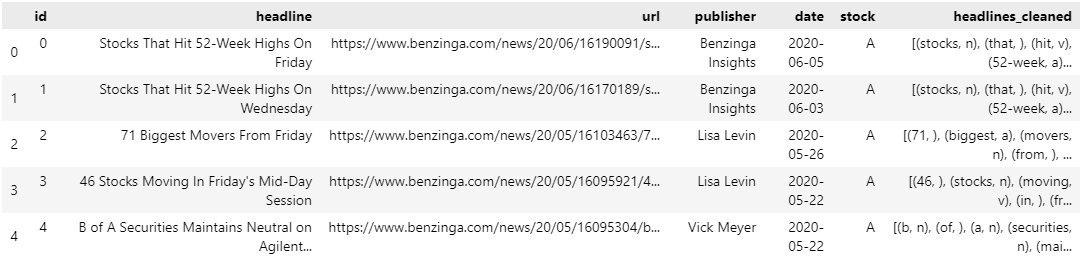
\includegraphics[scale=0.54]{img/Ausschnitt_Zwischenergebnis.png}
    \caption{Zwischenergebnis nach Tokenization, POST und Kleinschreibung}
    \label{Zwischenergebis_1}
\end{figure}
\\
Im nächsten Schritt werden die Stopwords entfernt. Auf diesen Schritt folgt nun die Lemmatizierung mittels dem Wordnet Lemmatizer. Wordnet ist ein lexikalisch-semantisches Netz, das seit 1985 an der Princteon University entwicklet wird. Es verfügt über zusammenhänge zwsichen Wörtern  \citep{miller1995}, und ist die Grundlage für viele andere Lexika, wie bspw. SentiWordNet \citep{bacianella2010}. Durch das POST weiss die Lemmatizer Funktion, um welche Wortart es sich handelt, und kann demetsprechend das jeweilige Wort auf die jeweilige Wörterbuchform zurückführen. Zu Vereinfachung behandeln wir alle Wörter, die beim POST keiner Wortart zugeordnet werden konnten, wie Nomen. Dahinter steht die Überlegung, keine Wörter zu verlieren, die im späteren Verlauf durch das SentiWordNet mit einem Senitment belegt werden könnten. Wir entfernen anschließend erneut weitere Wörter, nämlich jene, die weniger als drei Buchstaben haben sowie solche, die aus Zahlen bestehen, also numerisch sind.\\
\begin{figure}[t]
    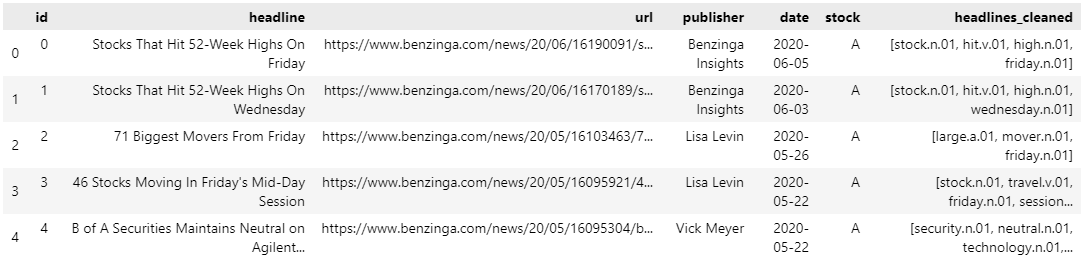
\includegraphics[scale=0.54]{img/Ausschnitt_Zwischenergebnis_2.png}
    \caption{Zwischenergebnis Snyset Format}
    \label{Zwischenergebnis_2}
\end{figure}
Mithilfe von SentiWordNet werden nun die Sentiments für jede Headline bestimmt. Dabei ergibt sich ein Senitment Score durch die Differenz zwischen poitivem Sentiment und negativem Sentiment. Diese Werte werden duch SentiWordNet geliefert und an die entsprechende Zeile ergänzt.

\section*{Integrieren}
Die bislang zwei Datensätze der Headlines mit dem Stockticker sowie dem SentimentScore und der Stockprices müssen, zur Verwendung im Modell, vereint werden. Dazu ergänzen wir jedem Eintrag des ersteren Datensatz mit dem \textit{open}-Kurswert und dem \textit{close}-Kurswert der jeweiligen Aktie am Tag der Veröffentlichung des Artikels. Um die Auswirkungen möglichst eindeutig zuweisen zu können, sollte ein entsprechend kleines Intervall verwendet werden. Um jedoch alle Auswirkungen zu erfassen, darf dieses auch nicht zu klein sein. Wir gehen davon aus, dass im Mittel, die Artikel nach Eröffnung des Aktienhandelsplatz und vor Schließung dessen publiziert werden. Dies ist auch auf der Webseite von Benzinga.com nach zu vollziehen. So wählen wir zu jeder Headline den Aktienkurs beim öffnen des Aktienhandelsplatz als Referenzwert und den Preis beim schließen als Zielvariable.  
%ToDo: discuss intervall of stockprices to headline publish
In dem nun vereinten Datensatz ergänzen wir zusätzlich noch, aus dem Datensatz berechenbare, Werte wie den \textit{Stockprice\_Change} und \textit{Senti\_Binary}. Die jeweiligen Werte des Stockprice\_Change bilden die Veränderung des Stockprices am Tag der Veröffentlichung der Headline vom Eröffnungskurs zum Kurs beim Schließen der Börse ab. Dabei nimmt die Spalte des Stockprice\_Change eine 1 an wenn sich der Wert der Aktie um mehr als 1\% steigert, -1 wenn die Aktie um mehr als 1\% fällt. Sonst eine 0, wir gehe davon aus, das die Aktie sich nicht Nennenswert geändert hat, bzw. die Headline als Ursache für die Veränderung des Aktienpreises ausgeschlossen werden kann. Die jeweiligen Werte des Senti\_Binary ergänzen den Datensatz um eine drei-tuple Betrachtung des Sentiment. Ist der verrechnete Sentiment, aus der Anzahl der Wörter mit Negativen und Positiven Sentiment, insgesamt positiv, also größer 0, so ist Senti\_Binary eine 1. Ist der Sentiment negativ, also kleiner 0, so ist der Senti\_Binary -1. Sonst 0.

\section*{Formatieren}
Wie bereits ausführlich beschrieben, wurde das Datumsformat auf yyyy-mm-dd reduziert. Weitere Formatierungen wurden nicht unternommen, die Daten verbleiben in der Form wie sie konstruiert wurden.

\section*{Ergebnis}
Der anfangs schon betrachtete Datensatz wurde nun um die bereinigten Überschriften, den Sentiment-Scores und den Aktienpreisen erweitert. Außerdem wurden die Einträge stark reduziert, unter anderem durch die Festlegung einer Datumsspanne zwischen dem 21.August 2019 und 31. Dezember 2020.\\ 
64456 headlines haben einen durchschnittlichen Sentiment von 0, davon haben 59718 weder einen positiven noch einen negativen Sentiment-Score. 
Hingegegen haben 97022 Headlines einen Sentiment-Score gesetzt der ungleich 0 ist. 45005 positive, 52017 negative. Dabei haben 50671 jeweils positive und negative zu bewertende Wörter.\\ \\
Es verbleiben 3722 Stocks und 76162 eindeutige Überschriften. Insgesamt also 14 Spalten auf 161478 Einträge.
Die folgende Abbildung bietet einen Überblick über den aktuellen Datensatz, welcher für das Modeling verwendet wird. Zu Übersichtszwecken wurden die Spalten \textit{url} und \textit{publisher} ausgeblendet.
\begin{figure}
    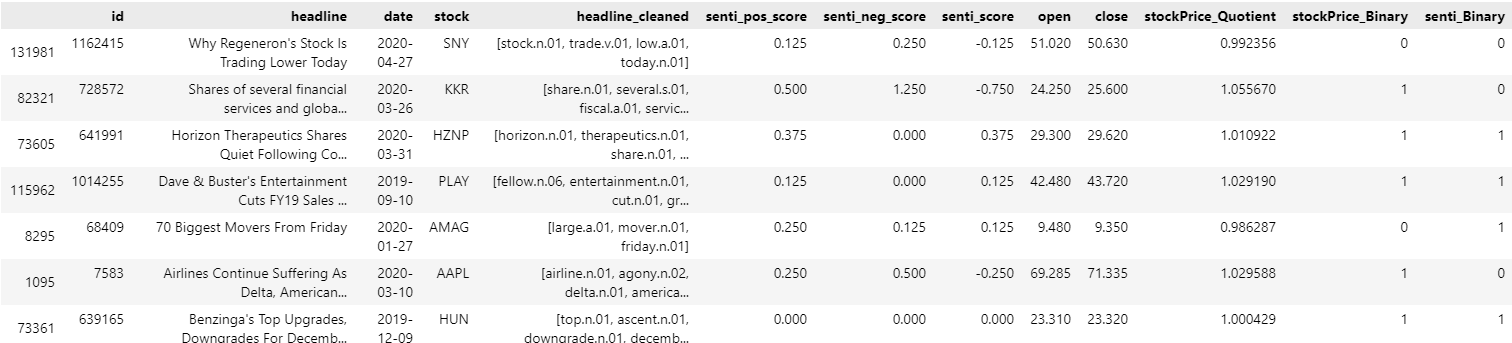
\includegraphics[width=1\textwidth]{img/dataSample7_constructed.png}
    \caption{Überblick über den konstruierten Datensatz, Sieben zufällige Einträge (url, publisher ausgeblendet)}
\end{figure} \\
Auch in den Überschriften selbst sieht man nach der Bereinigung einige Unterschiede. Ersichtlich ist, dass die Headlines vorrangig über die Lage des Handels berichten, so erscheinen Wörter wie ''Trade'' in Kombination mit ''high'' und ''low'' häufig. Jedoch erkennt man auch, dass einige Wörter wie ''company'', ohne weitere Aussagekraft, immer noch häufig verwendet werden. Vermutlich aufgrund des verwendeten, nicht spezifischen Stopword-Dictionary im Schritt des Stopword-Removal.
\begin{figure}
    \centering
    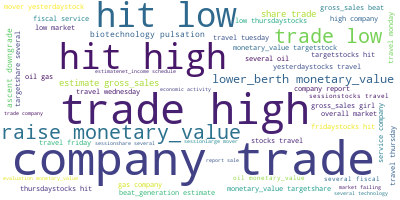
\includegraphics[scale=0.6]{img/wordcloud_afterCleaning.png}
    \caption{Top 50 Wörter im gesamten Datensatz, bereinigt}
\end{figure}
\chapter{Modeling}

Unsupervised um überblick zu schaffen.
Supervised mit Bewertungen.
\chapter{Evaluation}

Bewertung von Überschriften erfolgreich?
Zusammenhang von Überschriften und Unternehmens-"erflog" gegeben?
\chapter{Deployment}
Schlussendlich sollen die Ergebnisse des Modells den Unternehmen und den privat Anlegern zur Verfügung stehen.
Es soll Möglich sein, die Vorhersage des Modells zur Entwicklung des Aktienpreises schnell und unkompliziert bei Eingabe einer Headline zu erhalten.
Dies bietet sowohl den Unternehmen als auch den privat Anlegern den Vorteil eine objektive, datenbasierte Einschätzung der veröffentlichten Headline in ihre Entscheidungen am Markt einfließen zu lassen.

\section{Strategie}
Um eine möglichst einfache Handhabung zu gewährleisten, wird die Anwendung einfach gehalten: Eine Eingabe, eine Ausgabe.
Um außerdem den Unternehmen die Möglichkeit zu bieten, die Vorhersage in deren Unternehmensprozesse einzubinden, wird eine serverbasierte Anwendung erstellt, die Ihren Dienst über eine Schnittstelle zur Verfügung stellt. Denkbar ist es, dass Unternehmen neue Aktiennews automatisch sammeln und stetig durch das Modell bewerten lassen. So erhalten Unternehmen schnelles Feedback zu negativen Nachrichten und können entsprechend reagieren.\\
Durch die einfache API ist es ebenfalls möglich ein Grafisches-User-Interface zu entwickeln und auf die API zu legen, so können auch die private Anleger durch die Lösung erreicht werden.
Allerdings ist die Auslieferung und die Gestaltung der GUI nicht Teil dieser Studienarbeit.\\
Erreichbar die API durch einen HTTP-POST auf \textbf{/predict}.
Übergeben Sie die Headlines als Liste von Strings per \textit{POST, application/json} in folgender Form:
\begin{verbatim}
{
    'headlines': [
        'Dies ist eine Headline.', 
        'Dies ist noch eine Headline!'
    ]
}
\end{verbatim}
Die Antwort erfolgt ebenfalls per JSON in folgender Form:
\begin{verbatim}
{
    'prediction': [-0.627, 0.9965], 
    'stockChange': [-1, 1]
}
\end{verbatim}

\section{Implementation}
Nach den Schritten des Modelling, wird das trainierte Modell exportiert und statisch zur Verfügung gestellt.
Ein einfacher Flask-Server basierend auf Python lädt dieses und stellt eine API zur Verfügung.\\
Wird nun eine oder mehrere Headlines an die Anwendung gesandt, so durch läuft jeder dieser Überschriften die selben Pre-Processing Schritte wie im vorangegangenen Kapitel beschrieben. Nach folgend werden die entsprechenden numerische Werte aus der Headline berechnet und in das Modell eingesetzt. Das Modell liefert eine Vorhersage. Diese wird, zusammen mit der standartisierten Vorhersage (-1, 0 oder 1) als Response auf die Anfrage verpackt und versendet. \\
Zum produktiven Einsatz, insbesondere der Skalierung, wird die Verwendung eines Anwendungsserver empfohlen. Hier wird uWSGI verwendet, in kombination mit einem Nginx Webserver. Die Tatsache, dass der Server in einem Docker-Container läuft, erleichtert die Auslieferung und die Skalierung. Dennoch ist es möglich, die Anwendung ebenfalls lokal auszuführen. 

\section{Überwachen und Pflegen}
Um die stetige Weiterentwicklung des Modells zu ermöglichen, benötigt die Anwendung lediglich die exportierte Version des Modells, alle weiteren Schritte der API bleiben auch bei veränderten Modellen gleich. Dies ermöglicht das Austauschen und Verbessern des Modells. Außerdem ermöglicht die Tatsache der reinen containerbasierten Serveranwendung eine gute Skalierbarkeit. Das eigentliche Überwachen der Anwendung obliegt hier dem potenziellen Host.

% Bibliography
\newpage
\addcontentsline{toc}{chapter}{Bibliography} 
\bibliography{bibliography}

% Appendix (if required...)
% \appendix

% End
\end{document}